This chapter starts with hardware (mobile robot) used in the thesis. It explains the procedure adopted for base frame transformations of all sensors. Furthermore, proposed implementation, data acquisition process and results has been covered.

\section{Setup}
Mobile platform used for this scope of work is TurtleBot2e \cite{turtlebot2}. A 2nd generation robot of turtlebots family also known as Kobuki. The robot is equipped with 2D \acrshort{lidar}, Picocam and Genius-Widecam(F100) as shown in figure \ref{fig:turtlebot}.
\begin{figure}[h!]
	\centering
	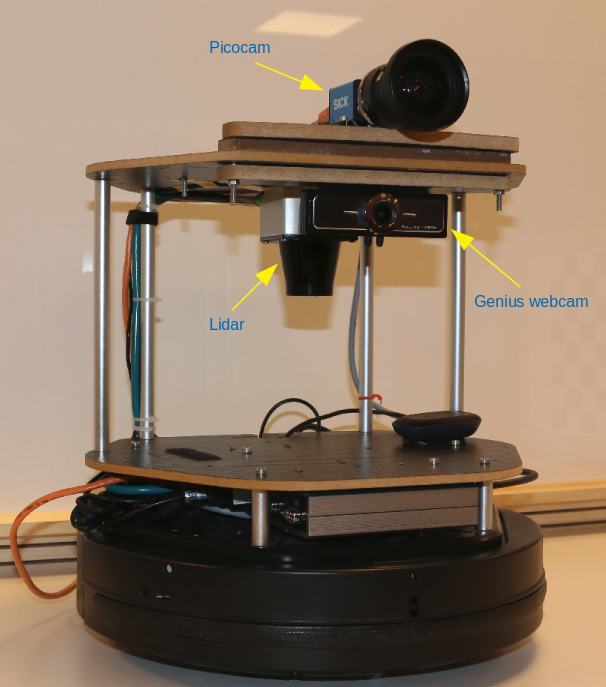
\includegraphics[width=0.62\textwidth]{turtlebot}
	\caption{Robot (turtlebot2) equipped with \acrshort{lidar}, picocam, genius widecam.}
	\label{fig:turtlebot}
\end{figure}
\subsection{Base frame transformation}
In order to compare the odometry results from all three sensors a common base is required. Therefore base-frame transformations is done with respect to \acrshort{lidar} center as reference frame. The procedure used a 2D chessboard placed at fixed distance of 1000 mm from \acrshort{lidar} and OpenCV software (e.g solvePnP algorithm) to calculate first extrinsic (R,t) parameters with respect to chessboard as base frame and then they transferred with respect to \acrshort{lidar} as base frame. An illustration of procedure is given in figure \ref{fig:transformation}. The result is shown in \ref{section:A.3}.
\begin{figure}[h!]
	\centering
	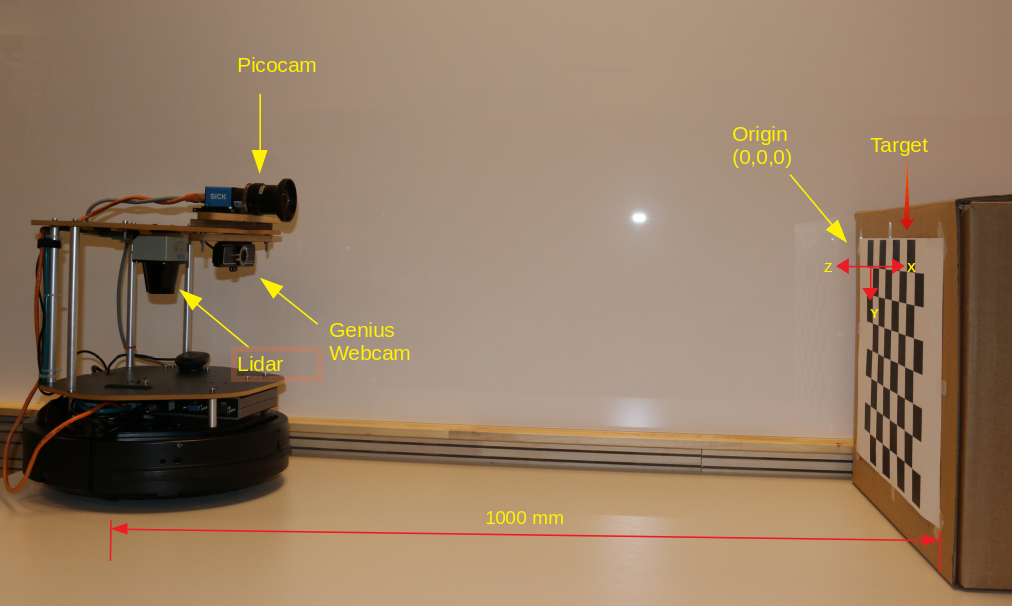
\includegraphics[width=1.0\textwidth]{frame_transformation}
	\caption{Setup to calculate base frame transformations}
	\label{fig:transformation}
\end{figure} 

\subsection{Implementation}
The software implementation of all three algorithms for both cameras along with \acrshort{lidar} odometry is shown in figure \ref{fig:implementation}. There are three types of raw data acquired for every experiment which is in form of stream container. The driver workers for each sensors then processed the data in the useful format. The figure \ref{fig:implementation} shows how raw data is processed to algorithm compatible form (e.g \textit{opencvuncompressed} image for \acrshort{vo} and \textit{scan} in case of \acrshort{lidar} odometry) and fed as the input to respective algorithms. The frequency for picocam and webcam was set as 18 and 30 frames per second respectively. For evaluation purpose the raw data is first collected and then fed to odometry algorithms. The output from all odometry algorithms is in from of position and orientation of the sensors at all timestamps and then transformed to the base frame (\acrshort{lidar} origin). The results is then compared with \acrshort{lidar} odometry and ground truth data.
\begin{figure}[h!]
	\centering
	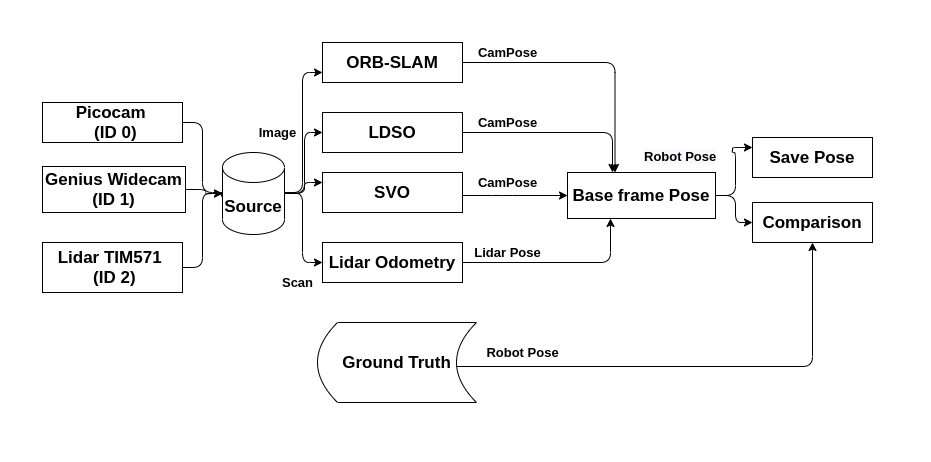
\includegraphics[width=1.0\textwidth]{implementation}
	\caption{Software implementation structure of \acrshort{vo} algorithms for the purpose of comparison}
	\label{fig:implementation}
\end{figure}


\subsection{Data acquisition}

How data is collected and figures of different sequences (with or w/o loop closing etc. ). warehouse setup figures. 
manual or autonomous navigation.

Some conditions or requirements of good data collection e.g. lighting etc. 

\section{Modifications and changes in implementation}
e.g with less features, less RANSAC iteration, window search size, no. of keyframes etc....
with figures.


\section{results}
